\documentclass[12pt]{article}
\setlength\headheight{14.5pt}
\title{Homework}
\author{Frederick Robinson}
\date{2 March 2010}
\usepackage{amsfonts}
\usepackage{fancyhdr}
\usepackage{graphicx}
\usepackage{amsthm}
\pagestyle{fancyplain}

\begin{document}



\lhead{Frederick Robinson}
\rhead{Math 368: Optimization}

   \maketitle

\setcounter{tocdepth}{2} 

\tableofcontents


\section{Problem 9.1}
\subsection{Question}
\begin{enumerate}
\item
 \[
  \mathcal{D}(\theta)= 
  \left\{\begin{array}{ll} 
  [0,2 \theta] & \mathrm{for\ }\theta \in [0,1/2) \\ 
  \ \! \![0,2-2 \theta]& \mathrm{for\ }\theta \in [1/2,1] \\ 
  \end{array} \right.
   \]
\item
 \[
  \mathcal{D}(\theta)= 
  \left\{\begin{array}{ll} 
  [0,1-2 \theta] & \mathrm{for\ }\theta \in [0,1/2] \\ 
  \ \! \![0,2-2 \theta]& \mathrm{for\ }\theta \in (1/2,1] \\ 
  \end{array} \right.
   \]
   \item
 \[
  \mathcal{D}(\theta)= 
  \left\{\begin{array}{ll} 
  [0,1-2 \theta] & \mathrm{for\ }\theta \in [0,1/2) \\ 
  \ \! \![0,2-2 \theta]& \mathrm{for\ }\theta \in [1/2,1] \\ 
  \end{array} \right.\]
   \item\[
   \mathcal{D}(\theta)= \{0,\theta\} \quad \mathrm{for\ } \theta \in [0,1]
   \]\end{enumerate}

\subsection{Answer}
\begin{enumerate}
\item This is a closed correspondence since given arbitrary $\theta$ we have $\mathcal{D}(\theta) $ closed. Moreover, since given arbitrary $\theta$ we have $\mathcal{D}(\theta) $ bounded we may surmise that this is a compact correspondence. 

It is both upper and lower semicontinuous. To show that this is the case (upper-semicontinuous) we merely note that for every. $\epsilon > 0$ there exists $\delta > 0$ such that $\theta \in B_\delta \theta_0 \cap \Theta \Rightarrow \Phi(\theta) \subset B_\epsilon \Phi(\theta_0)$. In particular $\theta = \theta_0 \pm \delta \Rightarrow \Phi(\theta_0 \pm \delta) \subset B_{3 \cdot \delta} \Phi(\theta_0)$. That is, given $\delta$ the condition is satisfied by taking $\epsilon = 3 \delta$

Now to establish lower semicontinuity we just need to show that for each $\epsilon >0$ there exists $\delta >0$ such that $\theta \in B_\delta \theta_0 \cap \Theta \Rightarrow \Phi(\theta_0) \subset B_\epsilon \Phi(\theta)$. The inverse relation works here though. That is; given $\delta$ taking $\epsilon = \delta / 3$ gives us  $\theta \in B_\delta \theta_0 \cap \Theta \Rightarrow \Phi(\theta_0) \subset B_{\delta/3} \Phi(\theta)$ as desired.

Since the correspondence is both upper and lower semicontinuous it is continuous.

\item This is a closed correspondence since given arbitrary $\theta$ we have $\mathcal{D}(\theta) $ closed. Moreover, since given arbitrary $\theta$ we have $\mathcal{D}(\theta) $ bounded we may surmise that this is a compact correspondence. 

It is easy to see that it is lower semicontinuous at each point of the region $[0,1/2) \cup (1/2,1]$ since on these regions it is compact, linear. It therefore remains only to check the point $\{1/2\}$.

However it is lower semicontinuous here too since for $\epsilon >0$ there exists $\delta >0$ such that $\theta \in B_\delta 1/2 \cap \Theta \Rightarrow \Phi(1/2) \subset B_\epsilon \Phi(\theta)$. In particular we may take any $\epsilon>0$ since for any $\theta \in B_\delta 1/2 \cap \Theta$ we have $\Phi(1/2) = \{0\} \subset B_\epsilon \Phi(\theta)$ as desired for any $\epsilon >0$.

The function is not upper semicontinuous since  there does not exist $\delta > 0$ such that $\theta \in B_\delta 1/2 \cap \Theta \Rightarrow \Phi(\theta) \subset B_\epsilon \Phi(1/2)$ for any $ \epsilon$. In particular $\theta = 1/2 \pm \delta \Rightarrow \Phi(1/2 \pm \delta) \subset B_{\epsilon } \Phi(1/2)$ for every epsilon. That is, the continuity condition fails to be satisfied at $\theta = 1/2$.

Since the correspondence is not upper and lower semicontinuous it is not continuous.


\item This is a closed correspondence since given arbitrary $\theta$ we have $\mathcal{D}(\theta) $ closed. Moreover, since given arbitrary $\theta$ we have $\mathcal{D}(\theta) $ bounded we may surmise that this is a compact correspondence. 

It is easy to see that it is upper semicontinuous at each point of the region $[0,1/2) \cup (1/2,1]$ since on these regions it is compact, linear. It therefore remains only to check the point $\{1/2\}$.

The function is upper semicontinuous since  there exists $\delta > 0$ such that $\theta \in B_\delta 1/2 \cap \Theta \Rightarrow \Phi(\theta) \subset B_\epsilon \Phi(1/2)$. In particular $\theta = 1/2 \pm \delta \Rightarrow \Phi(1/2 \pm \delta) \subset B_{3 \cdot \delta} \Phi(1/2)$. That is, given $\delta$ the condition is satisfied by taking $\epsilon = 3 \delta$. This is easy to see since $\Phi(1/2)=\{0\}$ so $B_{3 \delta} 0$ in particular includes all points in the image of $B_\delta 1/2$ under $\Phi$.

However it is not lower semicontinuity since for $\epsilon >0$ there does not exists $\delta >0$ such that $\theta \in B_\delta 1/2 \cap \Theta \Rightarrow \Phi(1/2) \subset B_\epsilon \Phi(\theta)$. That is; the continuity condition fails at $\theta = 1/2$ 

Since the correspondence is not upper and lower semicontinuous it is not continuous.

\item This is a closed correspondence since given arbitrary $\theta$ we have $\mathcal{D}(\theta) $ closed. Moreover, since given arbitrary $\theta$ we have $\mathcal{D}(\theta) $ bounded we may surmise that this is a compact correspondence. 

As this set is the union of finitely many (two) continuous functions: namely $f(\theta) = 0$ and $f(\theta) = \theta$ it is continuous and therefore upper and lower continuous. 

\end{enumerate}

\section{Problem 9.2}
\subsection{Question}
Let $\Theta = [0,1] = S$, and $h: S \times \Theta \to \mathbb{R}$ be defined by $f(x,\theta) =3+2x-3 \theta -5x \theta$. Here, $\mathcal{D}(\theta) = [0,1]$ for all $\theta$. Find $f^*(\theta)$ and $\mathcal{D}^*(\theta)$ for each value of $\theta$. Using the $f^*$ and $\mathcal{D}^*$ you have found, discuss why $f^*(\theta)$ is a continuous function and $\mathcal{D}^*(\theta)$ is a usc correspondence.
\subsection{Answer}
The relevant definitions are 
\[ f^*(\theta) = \sup\{f(x,\theta) : x \in \mathcal{D}(\theta) \} \in \mathbb{R}\]
\[\mathcal{D}^*(\theta) = \arg \max\{ f(x,\theta) : x \in \mathcal{D}(\theta) \} \subset \mathcal{D}(\theta) \subset \mathbb{R}^n\]

So in this case the members of $f^*(\theta)$ are those $x$ which maximize the given function on the unit interval, given $\theta$. In particular we have 
\[f(x,\theta_0) = 3+2x-3\theta_0-5x\theta_0 \]
Since this function is linear in $x$ it is maximized either at $0$ or $1$. For $\theta_0<2/5$ it is maximized at $1$ since the function is increasing in $x$. For $\theta_0 > 2/5$ it is maximized at $0$ and for $\theta_0 = 2/5$ it is maximized everywhere.

Therefore we have 
\[\mathcal{D}^*(\theta) = \left\{ \begin{array}{ll} 1& \theta<2/5 \\ \ \!\! [0,1] & \theta = 2/5 \\ 0 & \theta>2/5 \\ \end{array}\right.\]
and correspondingly we see by substituting these values in $f$ from above
\[f^*(\theta) = \left\{ \begin{array}{ll} 5-8\theta & \theta<2/5 \\ 9/5& \theta = 2/5 \\ 3-3\theta & \theta>2/5 \\ \end{array}\right.\]

Having computed these explicitly it is easy to see that $f^*$ is continuous and $\mathcal{D}$ is usc as desired. In particular $f^*$ is a piecewise defined, linear. Thus, since it agrees at the boundaries of each piece [check: 5-8(2/5)=9/5=3-3(2/5)] it is continuous. Finally, to confirm that $\mathcal{D}^*$ is usc as claimed we need only verify at $\theta = 2/5$ since the rest is linear. However, since at this point the entire codomain is the result of taking $\Phi(2/5)$  we see that for any $\epsilon > 0$ there exists $\delta > 0$ such that $\theta \in B_\delta \theta_0 \cap \Theta \Rightarrow \Phi(\theta) \subset B_\epsilon \Phi(\theta_0)$. In particular taking any $\delta >0$ fulfills this definition since, as every point of the codomain is in $ \Phi(\theta_0)$ clearly every point is in $B_\epsilon \Phi(\theta_0)$ for any $\epsilon>0$.

\section{Problem 9.3}
\begin{enumerate}
\item 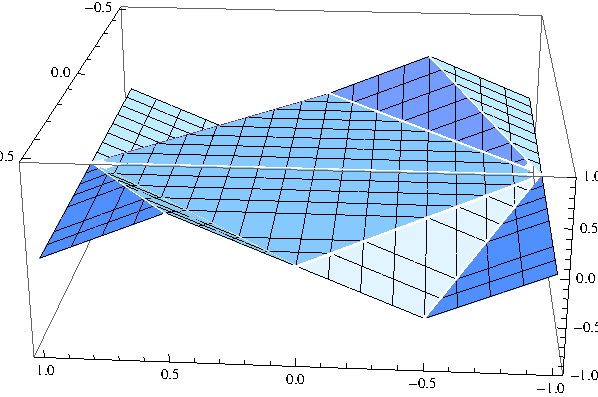
\includegraphics{sketch1}

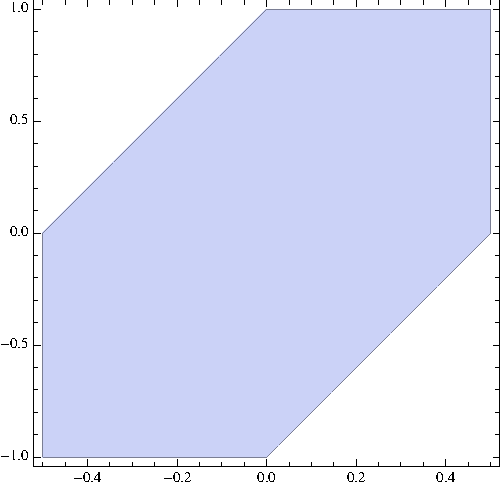
\includegraphics{sketch2}

$f$ is compact and $\mathcal{D}$ is continuous, and compact valued. Thus, the maximum theorem applies as desired.

\item Given $1/2>\theta>0$ the function $f$ has maximum at $x=1-\theta$ since for a fixed $\theta$ the maximum must occur at an endpoint of one of the piecewise defined regions by linearity. Then, by plugging in we find that the above is the correct (maximal) such endpoint.

On this set the function takes value $\theta$.

With $\theta=0$ the function is just constant valued (with value 0) so any value in $\mathcal{D}$ is a maximizing value.

Proceeding similarly for $0>\theta>-1/2$, we check each endpoint since linearity guarantees that one such point gives the maximum of the function for fixed $\theta$. In this manner we see that the maximum occurs at $|\theta|-1=x$ and the value of the function here is just $|\theta|$.

Now, sincethe maximizing points from above are not necessarily contained in $\mathcal{D}$ we must find which points of $\mathcal{D}$ maximize the function in these cases. However, a quick check reveals that they are all contained. (See first figure below)

To summarize we have
\[\mathcal{D}^*(\theta) = \left\{ \begin{array}{ll} 1-\theta & \theta<0  \\ \ \!\![-1,1] & \theta=0 \\ -\theta-1 & \theta>0 \\ \end{array}\right.\]
and correspondingly we see by substituting these values in $f$ from above
\[f^*(\theta) = \left\{ \begin{array}{ll} -\theta & \theta<0 \\ 0 & \theta = 0 \\ \theta & \theta>0 \\ \end{array}\right.\]

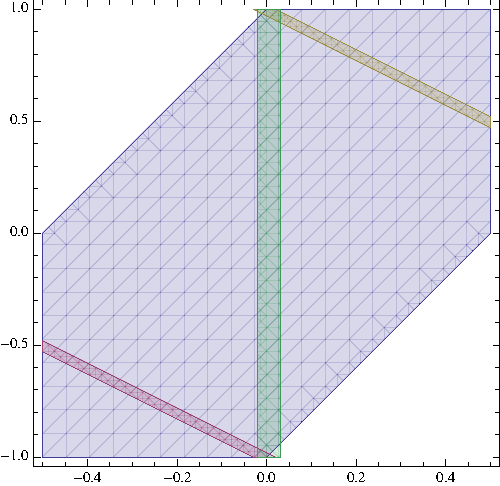
\includegraphics{sketch3}

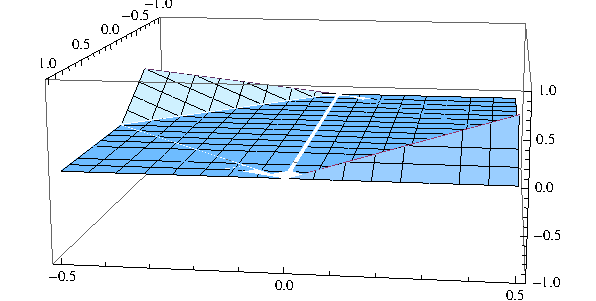
\includegraphics{sketch4}


\item The answer to both questions is yes. $f^*$ is continuous since it is just the absolute value function, which we know to be continuous. Moreover $\mathcal{D}^*$ is nonempty for every $\theta$ (it is defined above). Finally $\mathcal{D}^*$ is both lsc and usc on the relevant interval since as in the previous problem we know that at the ends ($\theta>0$ or $\theta<0$) it is continuous and we can verify $\theta=0$ by definition exactly as we did in the previous problem.
\end{enumerate}





\end{document}
